% Nama      : Bostang Palaguna
% NIM       : 13220055
% Tanggal   : Kamis, 17 Februari 2022
% Perintah  : salinlah file yang telah diberikan di kelas pada tanggal 17 Februari 2022
%%%%%%%%%%%%%%%%%%%%%%%%%%%%%%%%%%%%%%%%%%%%%%%%%

\documentclass[conference]{IEEEtran}
\IEEEoverridecommandlockouts

    % meng-import package yang digunakan
\usepackage{cite} % untuk mengutip referensi
\usepackage{amsmath,amssymb,amsfonts}
    % menulis pseudocode secara mandiri dengan LaTeX sangatlah menjemukkan!
%\usepackage{algpseudocode}  % untuk menulis pseudo-code
%\usepackage{algorithm} % untuk menulis pseudo-code
\usepackage{graphicx} % untuk memasukkan gambar
\usepackage{textcomp}
\usepackage{xcolor}
\usepackage{hyperref} % untuk menggunakan hyperlink 
\usepackage{float} % untuk menggunakan figure position specifier H -> agar posisi konsisten dengan urutan sourcecode

\def\BibTeX{{\rm B\kern-.05em{\sc i\kern-.025em b}\kern-.08em
    T\kern-.1667em\lower.7ex\hbox{E}\kern-.125emX}}
\begin{document}

%%%%%%%%%%%%%%%%%%%% JUDUL %%%%%%%%%%%%%%%%%%%%
\title
{
    Implementasi Algoritma Dijkstra Dalam
    Menemukan Jarak Terdekat Dari Lokasi Pengguna
    Ke Tanaman Yang Di Tuju\\
    {\footnotesize Dokumen LaTeX ini dibuat oleh \textbf{Bostang Palaguna(13220055)} }
}
\author
{
    Rafli F. Amanda\textsuperscript{$\ast$}
    , Reynaldo A. A. Putra\textsuperscript{$\dag$}
    , Muhammad Z. Fadhil\textsuperscript{$\ddag$}
    , Alifia Z. Ilmi\textsuperscript{$\S$}
    , Astrid N. Hasanah\textsuperscript{$\P$}
    \\
    \textit{School of Electrical Engineering and Informatics}
    \\
    \textit{Institut Teknologi Bandung}
    \\
    Bandung, Indonesia
    \\
    \{\textsuperscript{$\ast$}13219040, \textsuperscript{$\dag$}13219071, \textsuperscript{$\ddag$}18319012, \textsuperscript{$\S$}18319013, \textsuperscript{$\P$}18319014\}@std.stei.itb.ac.id
}

\maketitle


%%%%%%%%%%%%%%%%%%%% ABSTRAK %%%%%%%%%%%%%%%%%%%% 
\begin{abstract}
    Kebun Raya Purwodadi dengan luas area sekitar 85
    hektar ternyata kekurangan papan informasi yang menyebabkan
    pengunjung kerap kali kebingungan dalam mencari lokasi tanaman tertentu. Paper ini bertujuan untuk membuat simulasi
    dari algoritma yang dapat menentukan jarak terdekat antara
    pengunjung (pengguna program) dengan lokasi tanaman yang
    dituju. Algoritma yang digunakan adalah algoritma Dijkstra
    yang beroperasi secara menyeluruh (\textit{greedy}) untuk menguji
    seitap persimpangan (\textit{Vertex}) dan jalan (\textit{Edge}) pada Kebun
    Raya Purwodadi. Berdasarkan hasil simulasi dan pengujian,
    kompleksitas ruang dari program ini adalah $O(V)$ karena adanya
    pembentukan array yang berisi $V$ nodes untuk mencari heap minimum. Sementara, kompleksitas waktu dari algoritma tersebut
    adalah $O(V^2)$.
\end{abstract}

%%%%%%%%%%%%%%%%%%%% KATA KUNCI %%%%%%%%%%%%%%%%%%%%
\begin{IEEEkeywords}
    Dijkstra, Vertex, Edge, Tanaman.
\end{IEEEkeywords}

%%%%%%%%%%%%%%%%%%%% BAGIAN 1 : INTRODUKSI %%%%%%%%%%%%%%%%%%%%
\section{Introduction}
    Studi mengenai penggunaan algoritma Dijkstra dalam mencari jarak terdekat dapat diimplementasikan pada kasus pencarian tanaman pada Kebun Raya Purwodadi seperti yang telah
    dilakukan oleh Yusuf et al di tahun 2017 \cite{yusuf2017implementasi}. Paper ini bertujuan untuk melakukan simulasi kembali terhadap penelitian
    yang telah dilakukan dengan bahasa C serta mengevaluasi
    efisiensinya melalui perhitungan kompleksitas waktu dan ruang dengan analisis Big-O.
    
    Di Kecamatan Purwodadi, Kabupaten Pasuruan, terdapat
    salah satu kebun raya di Indonesia yang bernama Kebun
    Raya Purwodadi yang memiliki luas area hingga 85 hektar.
    Kebun raya sebagai fasilitas rekreasi dan penelitian ini ternyata
    kekurangan papan informasi yang seharusnya disediakan oleh
    pihak pengelola. Hal ini menyebabkan banyaknya pengunjung
    yang merasa kebingungan untuk mencari lokasi dari tanaman
    tertentu. Oleh karena itu, Yusuf et al (2017) memutuskan
    untuk membuat suatu aplikasi dengan memanfaatkan algoritma
    Dijkstra untuk membantu pengunjung Kebun Raya Purwodadi
    dalam mencari lokasi tertentu.
    
    Algoritma Dijkstra digunakan karena algoritma ini dapat
    beroperasi secara menyeluruh (algoritma greedy) terhadap
    semua alternatif fungsi serta durasi eksekusi yang lebih cepat
    jika dibandingkan dengan algoritma serupa, yaitu Bellman-Ford. Algoritma ini akan mencari jalur dengan 'biaya' atau cost terendah antara dua titik dengan membandingkan semua
    alternatif yang ada.
    
    Pada kasus ini, masing-masing persimpangan di Kebun
    Raya Purwodadi direpresentasikan sebagai vertex dan setiap
    jalan direpresentasikan sebagai edge. Rute terdekat yang didapatkan akan diperoleh dari pembobotan setiap vertex dan edge
    berdasarkan jarak antara titik pengguna dengan titik tujuan
    atau tanaman.

%%%%%%%%%%%%%%%%%%%% BAGIAN 2 : STUDI PUSTAKA %%%%%%%%%%%%%%%%%%%%
\section{Studi Pustaka}

\subsection{Algoritma Djikstra}

\begin{figure}[H]
    \centerline{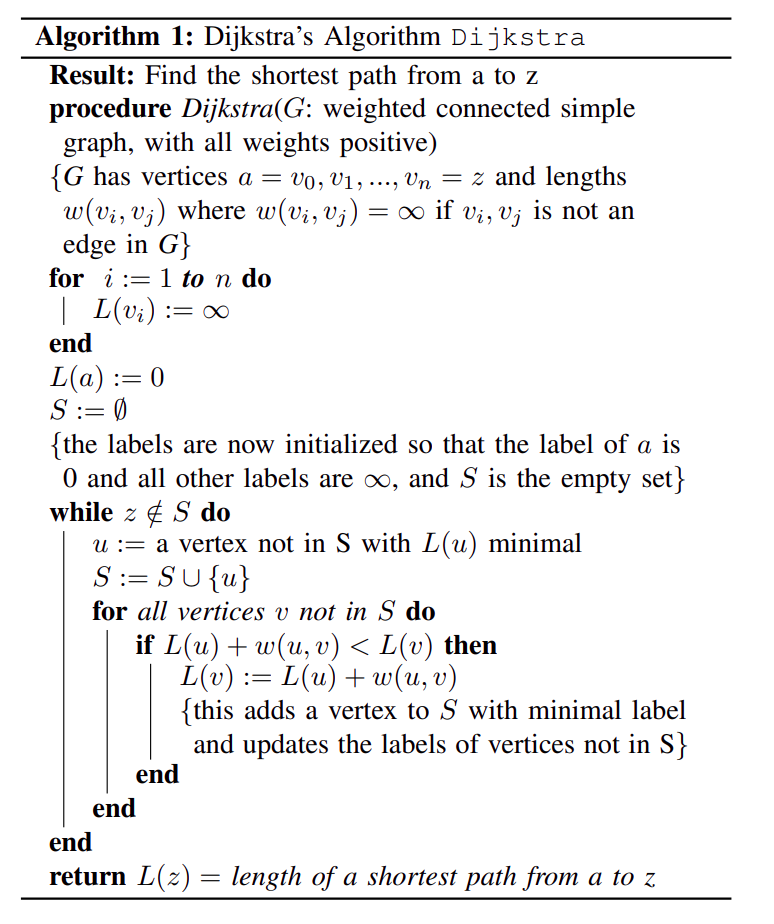
\includegraphics[width=0.4\textwidth]{./sources/algoritma_djikstra.png}}
    \caption{Pseudocode Algoritma Djikstra.}
    \label{fig1}
\end{figure}

    Algoritma Dijkstra adalah algoritma yang digunakan untuk
    menemukan jarak jalur terpendek antara dua \textit{vertice} pada
    \textit{graph} berbobot dan tidak berarah sederhana \cite{koshy2004discrete}. Berbobot
    berarti grafik memiliki \textit{edge} dengan suatu 'bobot' atau harga.
    Bobot dapat merepresentasikan jarak, waktu, atau apapun
    yang memodelkan koneksi antara kedua \textit{node}. Tidak berarah
    memiliki arti bahwa untuk setiap \textit{node} yang terhubung, kita
    dapat mendekati suatu \textit{node} dari kedua arah. Pendekatan Dijikstra juga memiliki asumsi bahwa bobot pada \textit{edge} memiliki
    nilai yang tidak negatif. Hal ini karena nilai bobot akan
    terus dibandingkan dan diambil nilai yang paling kecil. Ada
    banyak varian pada algoritma ini, namun pada percobaan
    ini digunakan varian dimana suatu node ditetapkan menjadi
    \textit{source node}. Dari \textit{node} inilah akan dicari jarak terpendek
    diantara node lain. Algoritma ini dicetuskan oleh Edsger
    Wybe Dijkstra, salah seorang tokoh ternama di bidang computer science \cite{dijkstra1959note}. Kompleksitas dari algoritma dijkstra adalah $O(n^2)$,
    dengan $n$ menyatakan jumlah \textit{vertice} dari \textit{graph} yang
    bersangkutan.

\subsection{Kebun Raya Purwodadi}

    Kebun Raya Purwodadi adalah kebun penelitian di Kecamatan Purwodadi, Jawa Timur. Ia juga dikenal dengan nama
    Hortus Ilkim Kering Purwodadi dan didirikan tanggal 30 Januari 1941 oleh Dr. L.G.M. Baas Becking. Sebagai cabang dari
    Kebun Raya Bogor, ia memiliki fungsi mengkoleksi tumbuhan
    yang hidup di dataran rendah kering. Sebagai Balai Konservasi
    Tumbuhan di bawah Pusat Konservasi Tumbuhan Kebun Raya,
    Kedeputian Bidang Ilmu Pengetahuan Hayati LIPI, kebun raya
    ini memiliki banyak tumbuhan yang dinaunginya. Dengan
    menggunakan algoritma Dijkstra, diharapkan ia dapat membantu pengunjung mencari tanaman tertentu maupun jarak
    yang paling optimal.

%%%%%%%%%%%%%%%%%%%% BAGIAN 3 : METODE PENELITIAN %%%%%%%%%%%%%%%%%%%%
\section{Metode Penelitian}
    Peneliti menggunakan beberapa tahap dalam penyusunan
    paper ini. Pertama, dilakukan pengkajian dan studi literatur
    dengan membaca referensi paper yang berkaitan dan memilih
    paper yang dapat menjadi acuan dalam penelitian yang dilakukan, sehingga dari pilihan topik dan tema yang berkaitan
    secara luas dapat dikecilkan menjadi sebuah paper yang mencakup mayoritas dari topik yang dibahas. Setelah ditemukan
    beberapa paper, dilakukan perangkuman untuk menentukan
    paper yang sesuai sekaligus membahas poin-poin penting
    dari paper yang ingin dicapai. Setelah kedua tahap tersebut
    dilewati, penentuan paper yang dijadikan prototype penelitian
    merupakan hal yang mudah dan menjadi titik pencapaian
    dalam studi literatur dan pemilihan topik dari prototype penelitian yang dilakukan.

    Setelah itu, tahap selanjutnya yang dilakukan oleh peneliti
    adalah pembuatan prototype berupa program yang ditulis
    dalam bahasa C. Pembuatan prototype berupa kode ini dilakukan terus-menerus dengan menggunakan metode trial and
    error sehingga perlu dilakukan revisi hingga protoype kode
    yang dibuat dapat mendapatkan output yang optimal dan
    sesuai dengan spesifikasi yang diharapakan. Tahap terakhir
    penelitian adalah pemaparan kode yang berhasil dijalankan tersebut ke dalam paper.

    \begin{figure}[H]
        \centerline{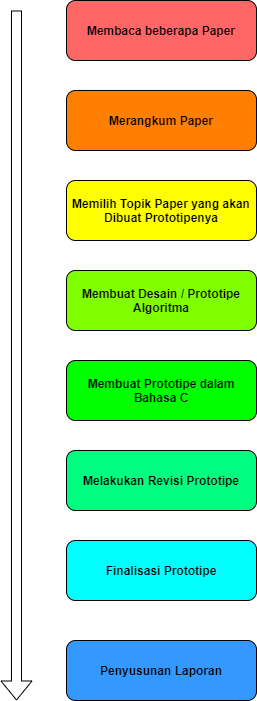
\includegraphics[width=0.15\textwidth]{./sources/metodologi_penelitian.png}}
        \caption{Skema Metodologi Penelitian.}
        \label{fig2}
    \end{figure}

%%%%%%%%%%%%%%%%%%%% BAGIAN 4 : IMPLEMENTASI DAN PENGUJIAN %%%%%%%%%%%%%%%%%%%%
\section{Implementasi dan Pengujian}

\subsection{Implementasi Graph pada Array dalam Bahasa C}

    Program akan dimulai dengan pembacaan file bernama
    \textit{listtanaman.txt}. File tersebut akan menyimpan informasi mengenai semua nama tanaman yang bersangkutan. Setelah pembacaan tersebut, akan dicari informasi mengenai bobot graph
    yang menghubungkan \textit{node}. Informasi ini disimpan di dalam
    matriks segitiga bawah kiri didalam file \textit{jarakantarpohon.txt}
    yang juga dibuka saat program dijalankan. Matriks menggambarkan bobot antara jarak dua \textit{node} tanaman sekali saja karena
    pemodelan \textit{undirected graph} yang memiliki jarak sama baik
    dari $a$ ke $b$ maupun $b$ ke $a$. Nilai $-1$ akan menggambarkan
    bagian node yang tidak terhubung sama sekali dalam graph 
    dan juga dinyatakan dalam suatu variabel bernama $int_max$
    (Jaraknya sebesar tak hingga). Nilai jarak terpendek akan
    disimpan dalam array tersebut selagi program berjalan.

\subsection{Implementasi Algoritma Dijkstra dalam Bahasa C}

    alam implementasi algoritma, abstraksi dengan menggunakan pseudocode dapat dibagi menjadi dua buah fungsi dan
    satu program utama. Fungsi yang digunakan adalah fungsi
    printgraph (Fungsi Graph) untuk memunculkan graph berukuran $n \times n$ ke layar pengguna. Algoritma dari fungsi tersebut
    dapat dilihat pada bagian di bawah ini:

    \begin{figure}[H]
        \centerline{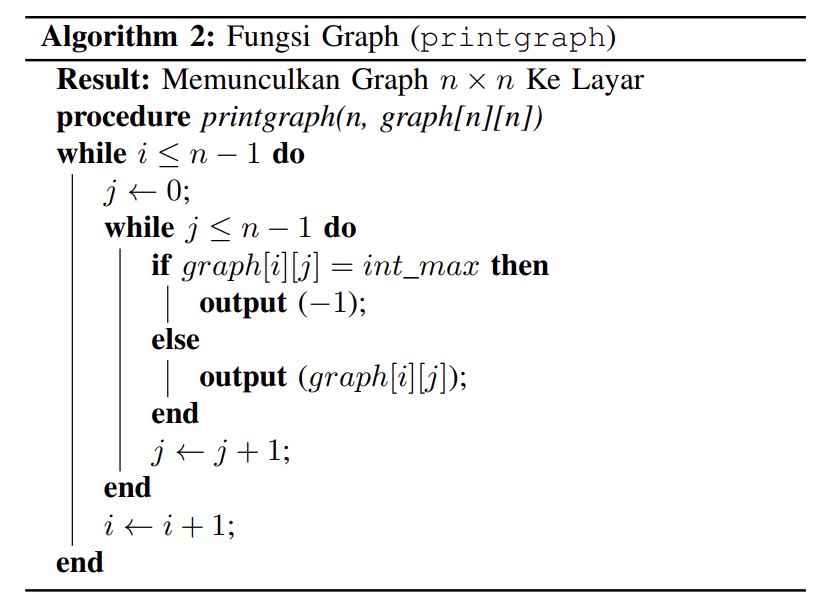
\includegraphics[width=0.4\textwidth]{./sources/printgraph.png}}
        \caption{Pseudocode fungsi \textit{printgraph}.}
        \label{fig3}
    \end{figure}

    Fungsi kedua yang digunakan adalah fungsi pencari indeks
    pada array yang akan diproses dengan menggunakan pendekatan algoritma Dijkstra. Abstraksi fungsi yang digunakan
    dapat dilihat pada bagian berikut ini:

    \begin{figure}[H]
        \centerline{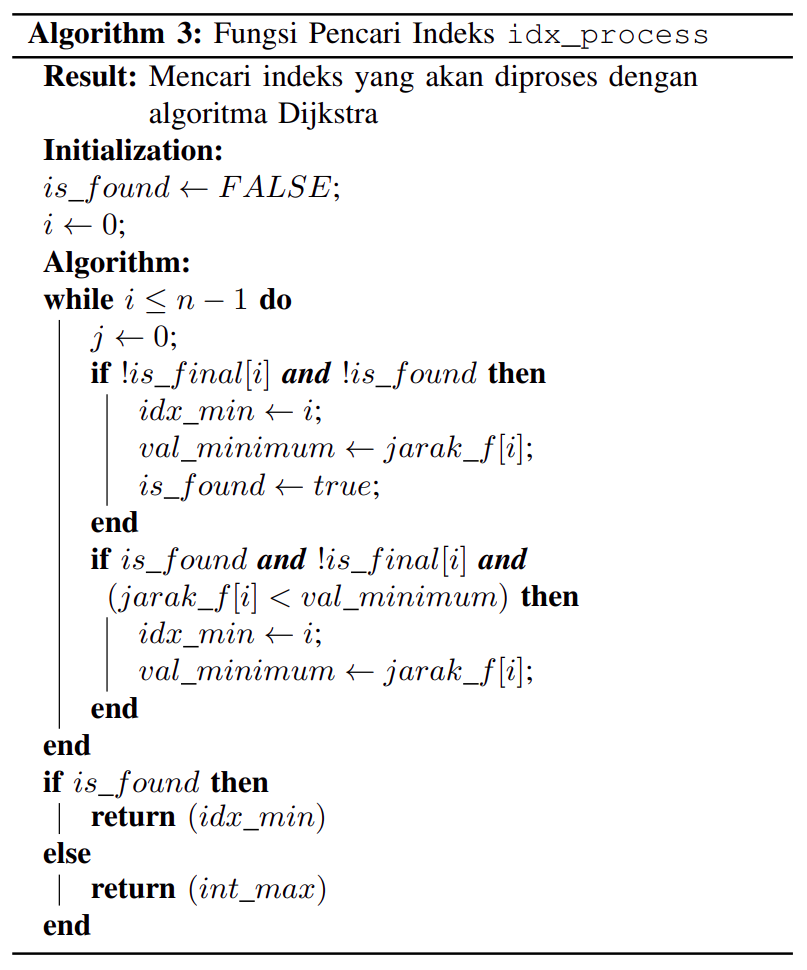
\includegraphics[width=0.4\textwidth]{./sources/idx_process.png}}
        \caption{Pseudocode fungsi \textit{idxprocess}.}
        \label{fig4}
    \end{figure}

    Program utama akan membaca file database tanaman
    beserta jarak masing-masing tanaman dan akan mencetak
    daftar tanaman yang berada di Kebun Raya Purwodadi.
    Kemudian, program akan menerima input salah satu tanaman
    terdekat dari pengguna sebagai penanda posisi awal pengguna.
    Setelah itu, program akan kembali menerima input posisi
    tanaman tujuan dan memproses pencarian rute terdekat dengan
    algoritma Dijkstra. Rute yang diperlukan akan ditampilkan
    dalam bentuk list nama tanaman yang harus dilalui pengguna
    dan menampilkan jarak antara kedua tanaman tersebut.
    Implementasi algoritma dalam abstraksi tersebut dapat dilihat
    pada gambar di bawah ini:
     
    \begin{figure}[H]
        \centerline{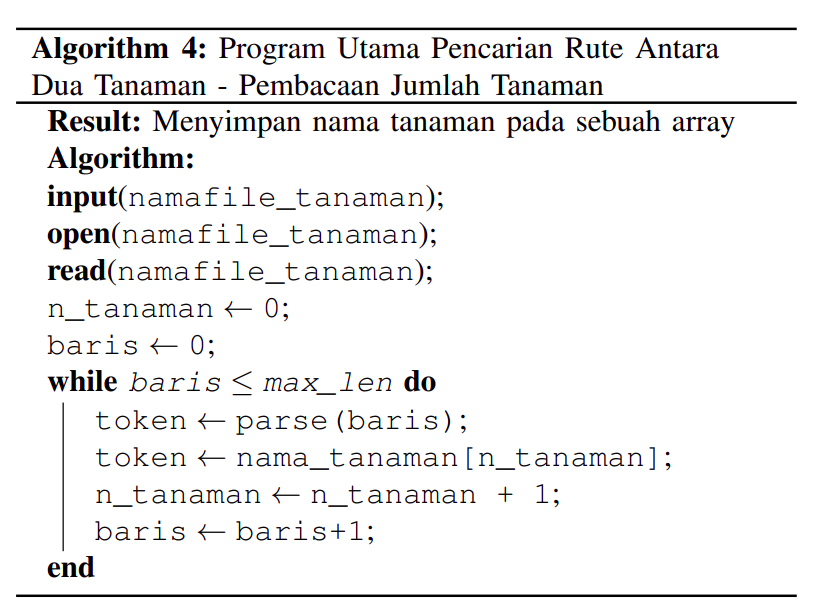
\includegraphics[width=0.4\textwidth]{./sources/bacaJumlahTanaman.png}}
        \caption{Pseudocode pembacaan jumlah tanaman.}
        \label{fig5}
    \end{figure}  

    Setelah pembacaan jumlah tanaman dari file, maka diperlukan graph atau jarak antar tanaman yang akan menjadi dasar
    perhitungan dari pencarian rute terdekat. Proses memasukkan
    graph dapat dilihat pada algoritma berikut ini:

    \begin{figure}[H]
        \centerline{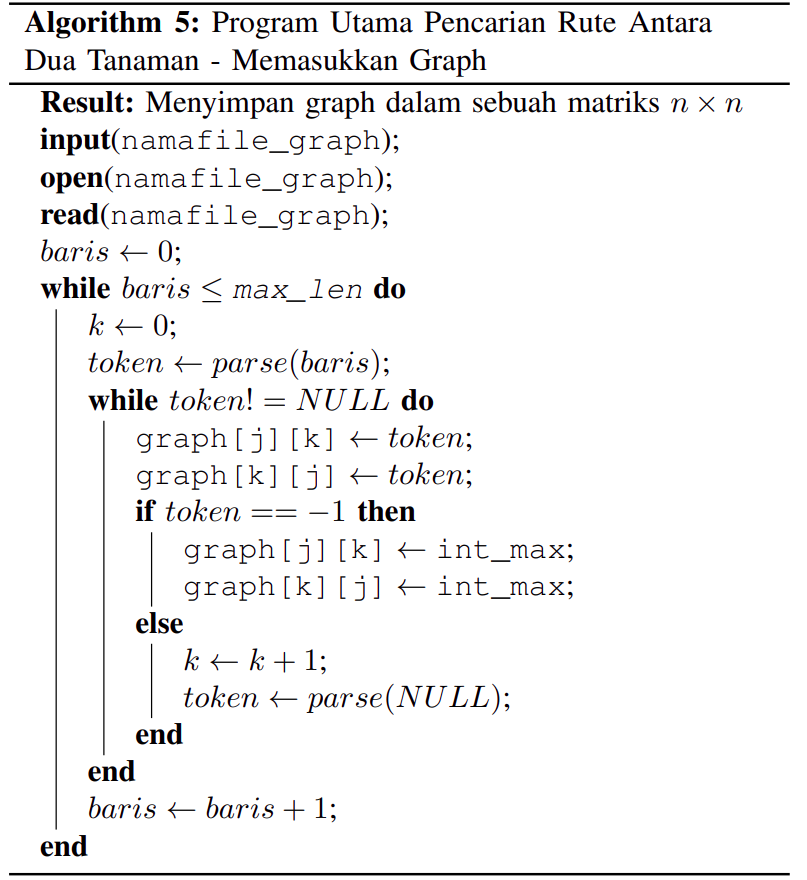
\includegraphics[width=0.4\textwidth]{./sources/masukkanGraph.png}}
        \caption{Pseudocode prosedur memasukkan graph.}
        \label{fig6}
    \end{figure}  

    Setelah data yang dibutuhkan dimasukkan, implementasi
    dari algoritma Dijkstra untuk pencarian rute terdekat adalah
    sebagai berikut:
    
    \begin{figure}[H]
        \centerline{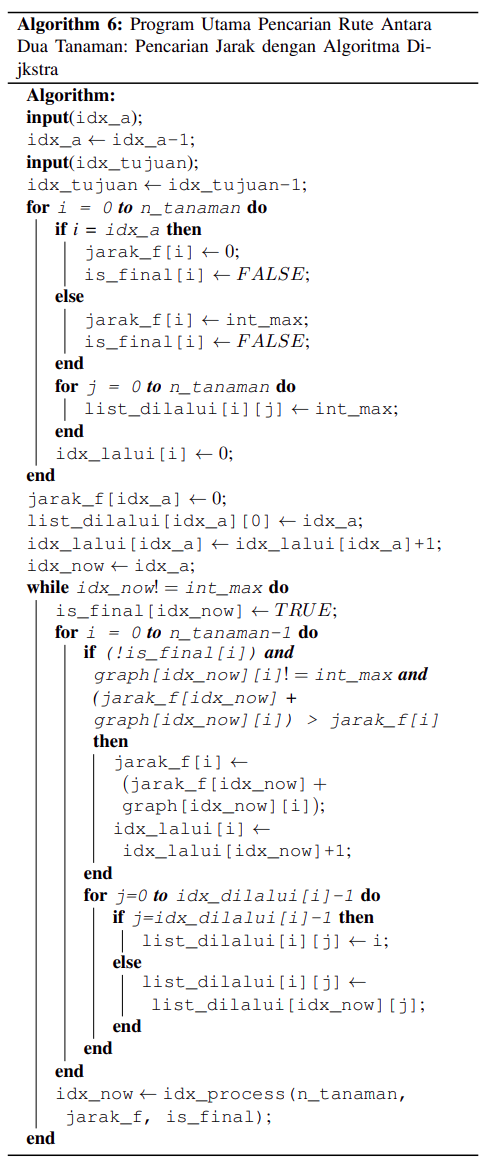
\includegraphics[width=0.4\textwidth]{./sources/cariJarak.png}}
        \caption{Pseudocode pencarian jarak dengan algoritma Djikstra.}
        \label{fig7}
    \end{figure} 

\subsection{Implementasi Program dalam Bahasa C}
    Implementasi program dalam bahasa C dapat dilihat
    pada \href{https://github.com/ReynaldoAverill/
    Tugas7PMC}{repository berikut}.

\subsection{Perhitungan Kompleksitas Waktu}
    Kompleksitas dari program ini dengan notasi kompleksitas
    Big O adalah $O(n^2)$. Hal tersebut disebabkan pada loop
    program bagian \textit{for}, terdapat loop \textit{for} lain yang berjumlah
    dua loop (Terletak pada bagian \textit{assign} kondisi awal dan ketika
    program menjalankan algoritma Djikstra). Karena hal tersebut,
    akibatnya adalah kompleksitas waktu akan naik seiring dengan
    naiknya $n$ program yang dijalankan, namun tidak bersifat
    linear sehingga kompleksitas waktunya adalah $O(n^2)$. Grafik
    kompleksitas waktu dapat direpresentasikan pada gambar berikut :

    \begin{figure}[H]
        \centerline{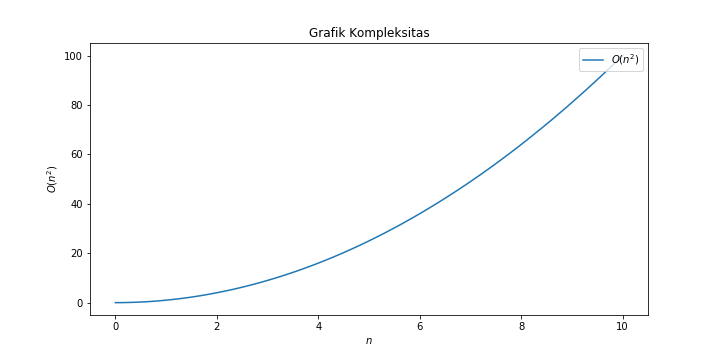
\includegraphics[width=0.5\textwidth]{./sources/onn.png}}
        \caption{Grafik kompleksitas waktu algoritma Djikstra.}
        \label{fig8}
    \end{figure}

\subsection{Perhitungan Kompleksitas Tempat}
    Matriks penyimpanan yang digunakan pada program ini
    memiliki ukuran terbesar $n \times n$, dengan nilai $n$ merepresentasikan banyak tanaman dalam file \textit{listtanaman.txt}. Program
    akan melalui grafik dan menyimpan nilai bobot antara \textit{node}
    sebesar matriks di atas, mengakibatkan program dengan kompleksitas $O(n^2)$. Hal ini dapat dilihat pada grafik kompleksitas
    tempat pada gambar berikut:

    \begin{figure}[H]
        \centerline{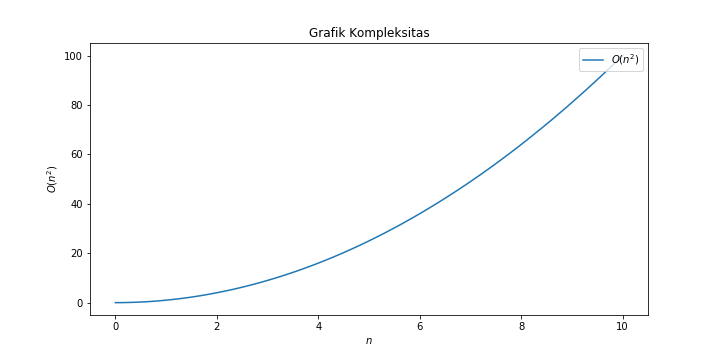
\includegraphics[width=0.5\textwidth]{./sources/onn.png}}
        \caption{Grafik kompleksitas ruang algoritma Djikstra.}
        \label{fig9}
    \end{figure}

\section{Kesimpulan}

    Pada perhitungan Jarak Terdekat dalam suatu lokasi atau ruang dapat diimplementasikan penggunaan Algoritma Djikstra
    dalam perhitungannya untuk mencapai suatu target pada ruang tersebut dari suatu titik. Terbukti dari penelitian Kebun Raya
    Purwodadi untuk menentukan Tanaman yang ingin dituju.

%%%%%%%%%%%%%%%%%%%% BIBLIOGRAFI %%%%%%%%%%%%%%%%%%%%

\bibliographystyle{IEEEtran}
\bibliography{referensi}

\end{document}


% referensi belajar
        % 1. kenapa kutipan muncul (?) 
    % https://tex.stackexchange.com/questions/63852/question-mark-or-bold-citation-key-instead-of-citation-number#:~:text=What%20does%20a%20question%20mark%20mean%20It%20means,so.%20Missing%20citations%20show%20up%20differently%20in%20biblatex
        % 2. menulis pseudo-code di LaTeX
    % https://tex.stackexchange.com/questions/163768/write-pseudo-code-in-latex
    % https://en.m.wikibooks.org/wiki/LaTeX/Algorithms
    % https://www.overleaf.com/learn/latex/Algorithms

% catatan
    % 1. BibTeX untuk kutipan diperoleh dari google scholar
    % 2. Gambar dibuat dengan menggunakan draw.io dan inkscape
        % sebelum import sebagai pdf_latex, pilih object to path terlebih dahulu pada tab path  